\tikzset{%
    add/.style args={#1 and #2}{
        to path={%
 ($(\tikztostart)!-#1!(\tikztotarget)$)--($(\tikztotarget)!-#2!(\tikztostart)$)%
  \tikztonodes},add/.default={.2 and .2}}
}  


\tikzset{%
  mark coordinate/.style={inner sep=0pt,outer sep=0pt,minimum size=2pt,
    fill=black,circle}%
}

\newcommand\pgfmathsinandcos[3]{%
  \pgfmathsetmacro#1{sin(#3)}%
  \pgfmathsetmacro#2{cos(#3)}%
}
\newcommand\LongitudePlane[2][current plane]{%
  \pgfmathsinandcos\sinEl\cosEl{\Elevation} % elevation
  \pgfmathsinandcos\sint\cost{#2} % azimuth
  \tikzset{#1/.estyle={cm={\cost,\sint*\sinEl,0,\cosEl,(0,0)}}}
}
\newcommand\LatitudePlane[2][current plane]{%
  \pgfmathsinandcos\sinEl\cosEl{\Elevation} % elevation
  \pgfmathsinandcos\sint\cost{#2} % latitude
  \pgfmathsetmacro\ydelta{\cosEl*\sint}
  \tikzset{#1/.estyle={cm={\cost,0,0,\cost*\sinEl,(0,\ydelta)}}} %
}
\newcommand\DrawLongitudeCircle[1]{
  \LongitudePlane{#1}
  \tikzset{current plane/.prefix style={scale=\R}}
  \pgfmathsetmacro\angVis{atan(sin(#1)*cos(\Elevation)/sin(\Elevation))} %
  \draw[current plane,thin,black]  (\angVis:1)     arc (\angVis:\angVis+180:1);
  \draw[current plane,thin,dashed] (\angVis-180:1) arc (\angVis-180:\angVis:1);
}%

\newcommand\DrawLatitudeCircle[1]{
  \LatitudePlane{#1}
  \tikzset{current plane/.prefix style={scale=\R}}
  \pgfmathsetmacro\sinVis{sin(#1)/cos(#1)*sin(\Elevation)/cos(\Elevation)}
  \pgfmathsetmacro\angVis{asin(min(1,max(\sinVis,-1)))}
  \draw[current plane,thin,black] (\angVis:1) arc (\angVis:-\angVis-180:1);
  \draw[current plane,thin,dashed] (180-\angVis:1) arc (180-\angVis:\angVis:1);
}%

\newcommand\DrawPointOnSphere[3]{%
\pgfmathsinandcos\sinLoM\cosLoM{#1}  
\pgfmathsinandcos\sinLaM\cosLaM{#2}
} 

\section{Orthodromie}
%\subsection{Aufgabenstellung}
%\begin{itemize}
  %\item Erstellung eines Entscheidungsnetzes auf der Erdkugel
  %\item Berechnung einer Orthodromie (Distanz in Meilen zwischen zwei Punkten auf der Erdkugel)
  %\item Erstellung der Koordinatendatei eines Sees
%\end{itemize}

\subsection{Problemanalyse}
\subsubsection{Berechnung einer Orthodromie}
Auf einer Kugel soll zwischen zwei Punkten die kürzeste Route bzw. die kürzeste
Verbindung gewählt werden, welche auch Orthodrome genannt wird. Die Orthodrome
ist immer ein Teilstück eines Grosskreises. Um die kürzeste Verbindung
zwischen den beiden Punkten $A$ und $B$ zu berechnen, werden zuerst die beiden
Vektoren vom Kugelursprung bis zu den Punkten ermittelt. Die beiden Vektoren
spannen dann mit dem Ursprung eine Ebene auf, deren Schnittlinie mit der
Kugeloberfläche (Sphäre) die Orthodrome darstellt. Da die zwei Punkte den Kreis
in zwei Kreisbogen separieren, wird nur der kürzere Distanz berücksichtigt.


Auf der Erdoberfläche werden die zwei Punkten in geographische Koordinaten,
Längen- und Breitengrad, angegeben. Die Erde wird dabei in 360 Längengrade und
180 Breitengrade aufgeteilt. Somit haben die beiden Punkte die folgende
Struktur: $A$ (\(\theta_1 , \phi_1\)) und $B$ (\(\theta_2 , \phi_2\)).

Für die Berechnung der Distanz benötigen wir die Längen- und Breitengrade der
zwei Punkte in Radian, welche dann in die Formel \eqref{eq:1} wie folgt
eingesetzt werden: \\
% Formel ArcCos(...)
\begin{equation}
\label{eq:1}
 \frac{360*60}{2 \pi} \arccos[\cos(\theta_1 - \theta_2) \cos(\phi_1) \cos(\phi_2)+\sin(\phi_1) \sin(\phi_2)]
 \end{equation}


%Die aufgespaltete Ebene lässt sich mit dem Vektorprodukt der beiden Punkten $A$ und $B$  berechnen. 


%Da die Erde eine Kugelform hat, werden die Koordinaten in Längen- und Breitengraden und die Distanz in Seemeilen angegeben. 
\begin{center}
  \begin{tikzpicture}
  \def\R{4} % sphere radius
  \def\Elevation{25} % elevation angle
  \def\angleLongitudeP{-110} % longitude of point P
  \def\angleLongitudeQ{-45} % longitude of point Q
  \def\angleLatitudeQ{30} % latitude  Q    ; 0 latitude of P 
  \def\angleLongitudeA{-20} % longitude of point A

  \pgfmathsetmacro\H{\R*cos(\Elevation)} % distance to north pole
  \LongitudePlane[PLongitudePlane]{\angleLongitudeP}
  \LongitudePlane[QLongitudePlane]{\angleLongitudeQ}
  \LongitudePlane[ALongitudePlane]{\angleLongitudeA}   

  \fill[ball color=white!10] (0,0) circle (\R); % 3D lighting effect
  \coordinate (O) at (0,0);
  \coordinate[] (N) at (0,\H);
  \coordinate[] (S) at (0,-\H);

  \DrawLongitudeCircle{\angleLongitudeP} % PLongitudePlane
  \DrawLongitudeCircle{\angleLongitudeQ} % QLongitudePlane
  \DrawLongitudeCircle{\angleLongitudeA} 
  \DrawLatitudeCircle{\angleLatitudeQ}
  \DrawLatitudeCircle{0} % equator
  \DrawLongitudeCircle{0}
  %setup coordinates P and Q
  \path[ALongitudePlane] (0:\R) coordinate (A);
  \path[ALongitudePlane] (32.5:\R) coordinate (A'); 
  \path[ALongitudePlane] (122.5:\R) coordinate (N');  
  \path[PLongitudePlane] (0:\R) coordinate (P);
  \draw[dashed,add= 1 and 0] (O) to  (P); 
  \path[QLongitudePlane] (\angleLatitudeQ:\R) coordinate (Q);
  \draw[dashed,add= 1 and 0] (O) to  (Q) ;
  \path[QLongitudePlane] (0:\R) coordinate (B);
  \draw [dashed] (O) --  (B) ;
  \draw [dashed] (O) --  (N) ;  

\foreach \v in {A,O,N,S,P,Q,A',B,N'} {\coordinate[mark coordinate] (v) at (\v);
\node [above] at (\v) {\v};} 
 \begin{scope}[ x={(P)}, y={(A')}, z={(N')}]     
          \draw[dashed,fill opacity=.3] circle (1);  
          \draw[blue] ( 0:1) arc (0:68:1) ;
          \draw[] ( 68:1) arc (68:115:1) ;
          \draw[] (-55:1) arc (-55:0:1);
          \draw[red,->](0,0,0)--(0,0,1); 
          \draw[red,->](0,0,0)--(0,1,0); 
          \draw[red,->](0,0,0)--(1,0,0);      
 \end{scope} 
\end{tikzpicture}   
\end{center}

\subsubsection{Erstellung eines Entscheidungsnetzes auf der Erdkugel}
Es soll ein Koordinatennetz mit den Knoten erstellt werden, auf welches dann
später die Berechnungen durchgeführt werden. Für die Erstellung des Netzes
benötigt man den Start- und Endpunkt als Eingabe. Die Anzahl der Knoten im Netz
werden von den weiteren zwei Eingaben m und n definiert, wobei m für die Anzahl
der Spalten und n für die Anzahl der Zeilen steht. Alle Punkte in diesem Netz
beinhalten ihre eigene Informationen über das Längen- und Breitengrad.

Der Abstand zwischen dem Start- und Endpunkt wird mittels der
Euklidischen-Abstand Verfahren ermittelt. Die Formel dafür lautet:

\begin{equation}
\label{eq:2}
e = \sqrt{ (\theta_2 - \theta_1)^2 + (\phi_2-\phi_1)^2}
\end{equation}

Somit sind die Spaltenlänge durch e/m und die Zeilenhöhe durch e/n definiert.
Da der Graph auch rotiert werden kann, braucht es eine Rotations-Matrix,
welches sich wie folgt zusammensetzt wobei $\alpha$ den Rotationswinkel im
Uhrzeigersinn darstellt.

\begin{equation}
\label{eq:3}
 M = \begin{pmatrix} \cos(\alpha) & -\sin(\alpha) \\ \sin(\alpha) &
 \cos(\alpha) \end{pmatrix} = \begin{pmatrix} \frac{\theta_2 - \theta_1}{e} &
 -\frac{\phi_2 - \phi_1}{e} \\ \frac{\phi_2 - \phi_1}{e} & \frac{\theta_2 -
 \theta_1}{e} \end{pmatrix}
\end{equation}

Am Ende erfolgt die Zusammenstellung des Koordinatennetzes für alle Knoten (i,
j) mit dieser Formel \eqref{eq:4}:

\begin{equation}
\label{eq:4}
Koordinatennetz = \begin{pmatrix} \frac{\theta_2 - \theta_1}{e} & -\frac{\phi_2 - \phi_1}{e} \\ \frac{\phi_2 - \phi_1}{e} & \frac{\theta_2 - \theta_1}{e} \end{pmatrix} * \begin{pmatrix}  \frac{e*i}{m} \\ \frac{\rho*e*j}{n} \end{pmatrix} + \begin{pmatrix}  \theta_1 \\ \phi_1 \end{pmatrix}
\end{equation}

Mit dieser Berechnung wird gewährleistet, dass die Zwischenknoten ein Rechteck
mit einem Gitternetz bilden, wobei die Start- und Endknoten genau in der Mitte
der gegenüberliegenden Seiten liegen.

In der Abbildung \ref{gridnet} wird gezeigt, wie so ein erstelltes
Koordinatennetz mit dem Startknoten (9.40 / 47.6) und dem Endknoten (9.64 /
47.58) aussieht.

\begin{figure}[h!]
\centering
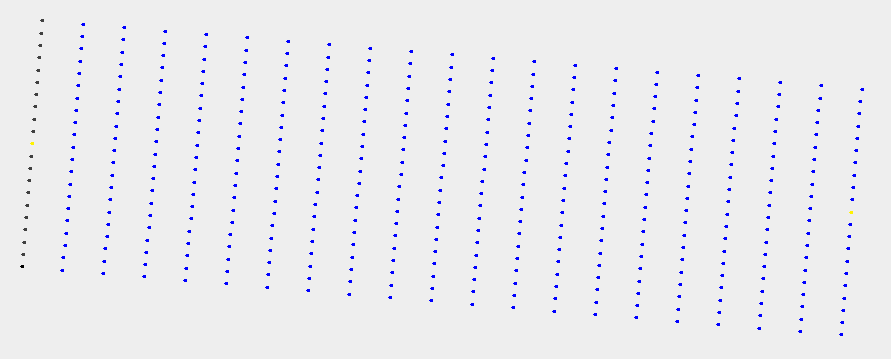
\includegraphics[width=1\linewidth]{img/gridNet}
\caption{Koordinatennetz}
\label{gridnet}
\end{figure}

\subsubsection{Seemeilen/Nautische Meilen} Damit Berechnungen einfacher werden, werden
hier nautische Meilen verwendet. Diese sind durch eine Bogenminute am Äquator
definiert und damit nur vom Radius des Planeten abhängig. Somit können unsere
Berechnungen genauso für andere Planeten gelten, einzig der
Umrechnungskoeffizient von Knoten nach $m/s$ muss angepasst werden.

\subsubsection{Aufspannen des Gitters für die Pfadberechnung} Das Gitter für die
Berechnung des schnellsten Pfades wird zwischen dem Start- und Zielpunkt so
aufgespannt, dass relativ-nördlich und -südlich des Startpunktes (und
Zielpunktes) jeweils eine gegebene Anzahl von Gitterpunkten erstellt wird, die
Gitterbreite. Vom Start- zum Zielpunkt hin werden auch eine gegebene Anzahl
Punkte verwendet, die Gitterlänge. Dieses Gitter bestehend aus Gitterbreite und
-länge, also $n\times m$, stellt den Suchbereich dar.

\subsubsection{Erstellung eines Entscheidungskernes in der dynamischen Programmierung}
Nach der Erstellung des Koordinatennetzes können die Orthodromie-Berechnungen auf die einzelnen Knoten durchgeführt werden. Wie auch oben in der dynamischen Programmierung beschrieben wurde, wird für jeden Knoten die Berechnung durchgeführt und mit der Knoten in der vorherigen Schicht eine Verbindung aufgebaut. \\
Grafisch dargestellt würde es ungefähr so aussehen:
\begin{figure}[h!]
\centering
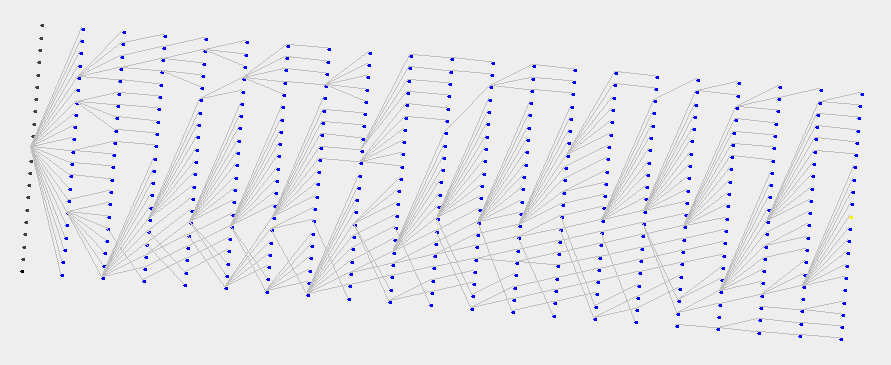
\includegraphics[width=1\linewidth]{img/gridNet_connections}
\caption{Koordinatennetz mit Verbindungen}
\label{gridnetConn}
\end{figure}
%% TikZ-Grafik mit Matrix


